\chapter{Task 2 --- First-Epoch Batch-Level Learning Analysis}
\label{ch:task2}

%-------------------------------------------------------

Task 2 asks for the training loss, training accuracy and F1-score of the
baseline plotted by batch during the first epoch (2--4 graphs), an
explanation of the learning behavior, and how the F1-score was
calculated. The baseline was trained for the full 10 epochs; this
chapter looks only at epoch 1, and Chapter \ref{ch:task3} covers all 10.

During the first epoch of the baseline (750 batches of 64 images), the
training loop recorded the loss, accuracy and macro-F1 of every batch
(Section \ref{sec:loop}). To keep the plots readable, the faint line
shows only every 5th batch, and the solid line is a 50-batch running
average over all batches. The per-batch macro-F1 is computed on the 64
predictions of that batch alone, with scikit-learn's
\texttt{f1\_score(average="macro")}, averaging over the digits present in
that batch's labels or predictions. A random batch of 64 occasionally
misses a digit entirely (8 of the 750 batches in this epoch), and that
digit is left out of the average instead of being counted as an F1 of
0. Since a batch has only about six images of each digit, one mistake
changes a class's F1 by a lot, so
Figure \ref{fig:epoch1-f1} also shows a cumulative macro-F1 computed over
every image seen so far in the epoch.

\begin{figure}[H]
    \centering
    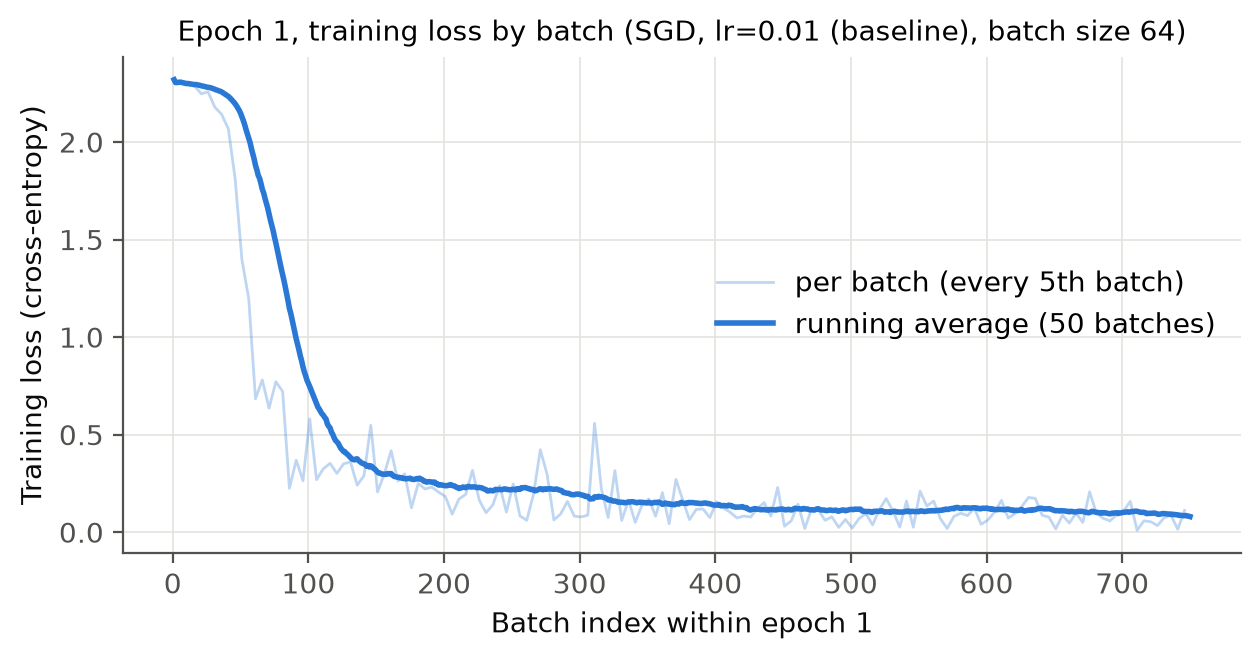
\includegraphics[width = 0.88\textwidth]{epoch1_loss.png}
    \caption[Epoch 1: training loss by batch.]%
    {Baseline (SGD, $\eta = 0.01$, batch size 64): training cross-entropy
    loss during the first epoch.}
    \label{fig:epoch1-loss}
\end{figure}

\begin{figure}[H]
    \centering
    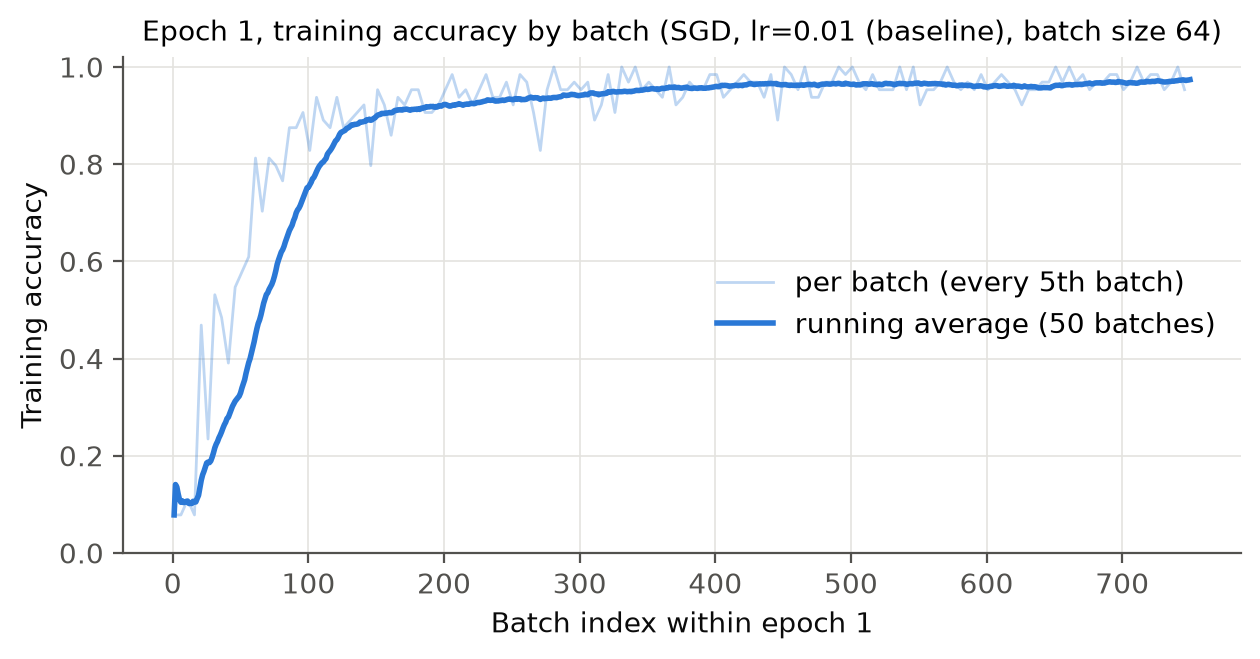
\includegraphics[width = 0.88\textwidth]{epoch1_accuracy.png}
    \caption[Epoch 1: training accuracy by batch.]%
    {Baseline: training accuracy of each batch during the first epoch.}
    \label{fig:epoch1-acc}
\end{figure}

\begin{figure}[H]
    \centering
    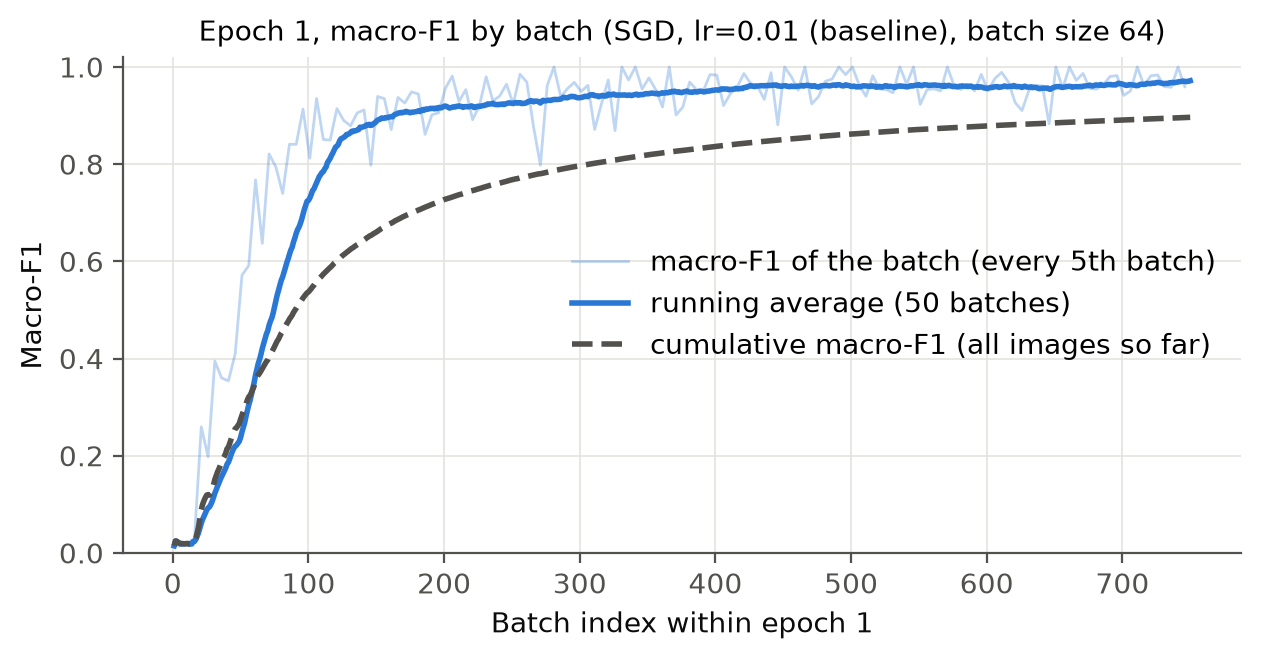
\includegraphics[width = 0.88\textwidth]{epoch1_f1.png}
    \caption[Epoch 1: macro-F1 by batch.]%
    {Baseline: per-batch macro-F1, its running average, and the
    cumulative macro-F1 over all images seen so far in the first epoch.}
    \label{fig:epoch1-f1}
\end{figure}

\textbf{Observation.} The first batch has a loss of 2.32 and an accuracy
of 7.8\%. This is what an untrained network should give: with random
weights, all 10 classes get about the same probability, so the loss is
close to $\ln 10 = 2.30$ and accuracy is close to the 10\% chance level.
The epoch then goes through three phases:

\begin{enumerate}
  \item Slow start (batches 1--40). The loss only goes from 2.32 to
        2.04. The gradients are small at first, and momentum needs a few
        steps to build up speed.
  \item Fast learning (batches 40--150). The loss falls quickly: the
        50-batch average is 2.15 at batch 50, 0.76 at batch 100 and 0.24
        at batch 200. Accuracy and macro-F1 rise together, and the
        running accuracy passes 90\% at batch 151. Most of the epoch's
        improvement happens in these hundred or so batches.
  \item Refinement (batches 150--750). Progress slows down and the
        curves flatten. By the end of the epoch, the running loss is 0.08
        and the running accuracy is 97.4\%.
\end{enumerate}

The per-batch curves stay noisy until the end (in the last 100 batches,
batch accuracy still varies between 92\% and 100\%) because each batch
is a different random sample of 64 images. Accuracy and macro-F1 follow
almost the same path: MNIST classes are nearly balanced, so no digit is
being ignored and the two metrics agree. The cumulative macro-F1 ends at
0.896, well below the late-batch values of about 0.97, because it still
includes the predictions from the start of the epoch when the network was
guessing.
